\begin{activity} \label{A:10.4.2} Let $f$ be the function defined by $f(x,y) = x^{1/3}y^{1/3}$.
    \ba
    \item Determine
    \[\lim_{h \to 0} \frac{f(0+h,0)-f(0,0)}{h}.\]
    What does this limit tell us about $f_x(0,0)$?



    \item Note that $f(x,y)=f(y,x)$, and this symmetry implies that $f_x(0,0) = f_y(0,0)$. So both partial derivatives of $f$ exist at $(0,0)$. A picture of the surface defined by $f$ near $(0,0)$ is shown in Figure \ref{F:10.4.Not_diff}. Based on this picture, do you think $f$ is locally linear at $(0,0)$? Why?
\begin{figure}[h]
\begin{center}
\resizebox{!}{2.5in}{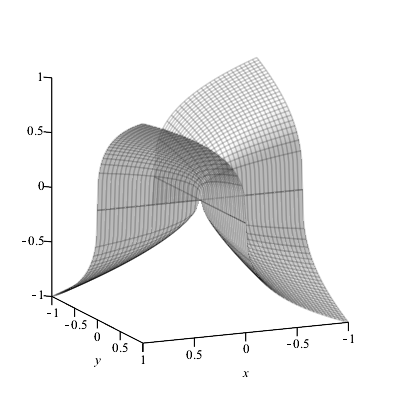
\includegraphics[trim=0cm 0.25cm 0.1cm 1.5cm,clip]{10_4_Not_diff}}
\end{center}
\caption{The surface for $f(x,y) = x^{1/3}y^{1/3}$.}
\label{F:10.4.Not_diff}
\end{figure}
%crop graphics in animate trim=<left> <bottom> <right> <top> (add clip with \includegraphics)



    \item Show that the curve where $x=y$ on the surface defined by $f$ is not differentiable at 0. What does this tell us about the local linearity of $f$ at $(0,0)$?



    \ea

\end{activity}
\begin{smallhint}

\end{smallhint}
\begin{bighint}

\end{bighint}
\begin{activitySolution}
\ba
\item For $f(x,y) = x^{1/3}y^{1/3}$, we have 
\[\lim_{h \to 0} \frac{f(0+h,0)-f(0,0)}{h} = \lim_{h \to 0} \frac{0}{h} = 0.\]
Since 
\[f_x(0,0) = \lim_{h \to 0} \frac{f(0+h,0)-f(0,0)}{h}\]
we have that $f_x(0,0) = 0$. 

\item The sharp folds in the graph of $f$ around $(0,0)$ would indicate that $f$ is not differentiable at $(0,0)$.  

\item Along the curve $y=x$ we have $g(x) = f(x,x) = x^{2/3}$. Now $g'(x) = \frac{2}{3x^{1/3}}$ is not defined at $x=0$, so $g$ is not differentiable at $0$. So we should expect that $f$ is not locally linear at $(0,0)$ and so is not differentiable there. 

\ea
\end{activitySolution}
\aftera
